\documentclass{llncs}
\usepackage{fullpage}
\usepackage{float}
\usepackage{tikz}
\usepackage{amsmath}
\usetikzlibrary{arrows, automata, positioning}

\usepackage{enumitem}
\usepackage{graphicx}
\usepackage{array}
\usepackage{pgfgantt}
\usepackage{booktabs}
\usepackage[utf8]{inputenc}

% Redefine las subsecciones para usar letras en lugar de números
\usepackage{titlesec}
\renewcommand\thesubsection{\alph{subsection})}

\begin{document}

\title{Planificación de tareas}

\author{Miguel Ángel Dorado Maldonado}
\institute{\email{miguelangeldorado10@uma.es} \\
TCIS. Universidad de Málaga.}

\maketitle

\vspace{1cm}

\section{Un proyecto viene especificado por el siguiente orden de precedencia de sus actividades:}

\begin{align*}
B &\longrightarrow C \\
A, B &\longrightarrow D \\
C, D &\longrightarrow E \\
A, B &\longrightarrow F \\
F &\longrightarrow G \\
E, G &\longrightarrow H \\
H &\longrightarrow I \\
\end{align*}

\begin{enumerate}

	\item[a)] Realice un diagrama con la programación de las actividades.

		\begin{figure}[H]
		\centering
		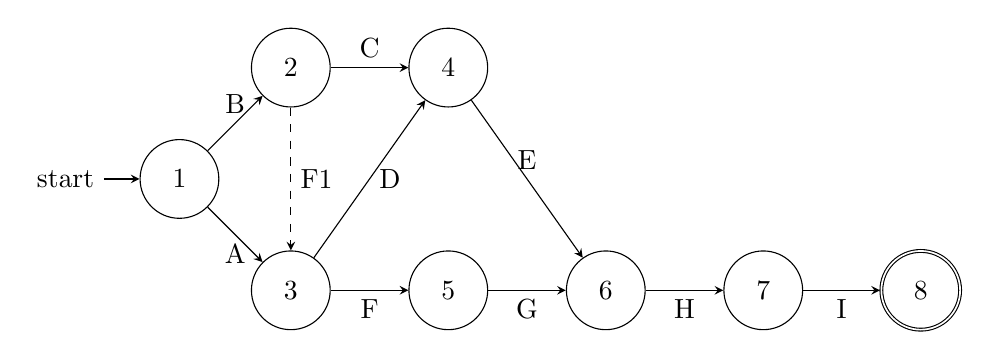
\begin{tikzpicture}[->, >=stealth, node distance=2cm, state/.style={circle, draw, minimum size=1cm}]

		\node[state, initial] (1) {1};
		\node[state] (2) [above right of=1] {2};
		\node[state] (3) [below right of=1] {3};
		\node[state] (4) [right of=2] {4};
		\node[state] (5) [right of=3] {5};
		\node[state] (6) [right of=5] {6};
		\node[state] (7) [right of=6] {7};
		\node[state, accepting] (8) [right of=7] {8};

		\path
		(1) edge node[above] {B} (2)
				edge node[below] {A} (3)
		(2) edge node[above] {C} (4)
				edge[dashed] node[right] {F1} (3)
		(3) edge node[below] {F} (5)
		 		edge node[right] {D} (4)
		(4)	edge node[above] {E} (6)
		(5) edge node[below] {G} (6)
		(6) edge node[below] {H} (7)
		(7) edge node[below] {I} (8);

		\end{tikzpicture}
		\caption{Diagrama de precedencia de actividades}
		\end{figure}

	\item[b)] Suponga el siguiente cuadro de duraciones para cada actividad.

		\begin{center}
		\begin{tabular}{|c|ccccccccc|}
			\hline
			$Actividad$ & $A$ & $B$ & $C$ & $D$ & $E$ & $F$ & $G$ & $H$ & $I$ \\
			\hline
			Duración (días) & 3 & 1 & 2 & 1 & 10 & 2 & 8 & 6 & 3 \\
			\hline
		\end{tabular}
		\end{center}
		Determine la duración del proyecto y su camino crítico.

				\begin{figure}[H]
					\centering
						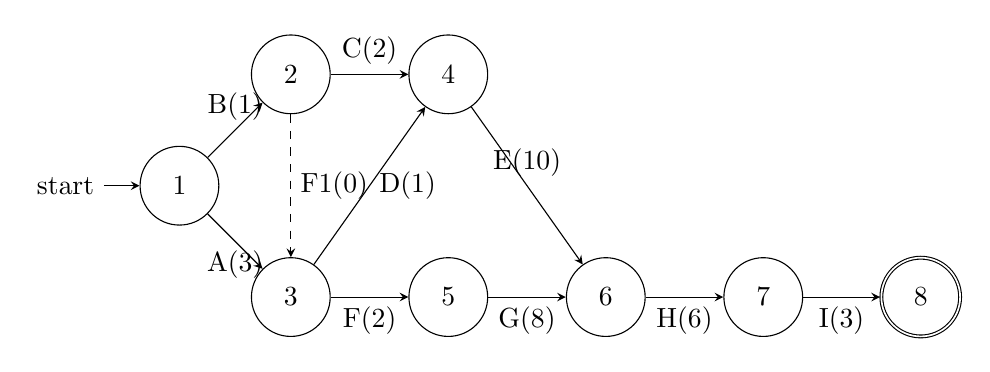
\begin{tikzpicture}[->, >=stealth, node distance=2cm, state/.style={circle, draw, minimum size=1cm}]

							\node[state, initial] (1) {1};
							\node[state] (2) [above right of=1] {2};
							\node[state] (3) [below right of=1] {3};
							\node[state] (4) [right of=2] {4};
							\node[state] (5) [right of=3] {5};
							\node[state] (6) [right of=5] {6};
							\node[state] (7) [right of=6] {7};
							\node[state, accepting] (8) [right of=7] {8};

							\path
							(1) edge node[above] {B(1)} (2)
									edge node[below] {A(3)} (3)
							(2) edge node[above] {C(2)} (4)
									edge[dashed] node[right] {F1(0)} (3)
							(3) edge node[below] {F(2)} (5)
									edge node[right] {D(1)} (4)
							(4)	edge node[above] {E(10)} (6)
							(5) edge node[below] {G(8)} (6)
							(6) edge node[below] {H(6)} (7)
							(7) edge node[below] {I(3)} (8);

						\end{tikzpicture}
					\caption{Diagrama de precedencia de actividades con duración}
				\end{figure}

				Conocidos los tiempos de duración de cada actividad, se calcula el camino crítico y la duración del proyecto por el método CPM. Para ello se calculan los tiempos de inicio early ($E_i$) y late ($L_i$) de cada actividad.

				\begin{center}
					\begin{tabular}{|@{\hspace{0.3cm}}c@{\hspace{0.3cm}}|@{\hspace{0.3cm}}c@{\hspace{0.3cm}}|@{\hspace{0.3cm}}c@{\hspace{0.3cm}}|}
						\hline
						$t$ & $E_i$ & $L_i$ \\
						\hline
						1 & 0 & 0 \\
						2 & 1 & 2 \\
						3 & 3 & 3 \\
						4 & 4 & 4 \\
						5 & 5 & 6 \\
						6 & 14 & 14 \\
						7 & 20 & 20 \\
						8 & 23 & 23 \\
						\hline
					\end{tabular}
				\end{center}


				Una vez calculados estos tiempos, es necesario obtener los tiempos de holgura para encontrar el camino crítico. La holgura ($H_{ij}$) se calcula como $L_j$ - $E_i$ - $D_{ij}$, donde $L_j$ es el tiempo de terminación más tardío de la actividad, $E_i$ es el tiempo de inicio más temprano de la actividad y $D_{ij}$ es la duración de la actividad. $R_{ij}$ representa los nodos que representan inicio y fin de la actividad.

				\begin{center}
					\begin{tabular}{|c|c|c|c|c|c|c|}
						\hline
						Tarea & $R_{ij}$ & $D_{ij}$ & $E_i$ & $L_j$ & $H_{ij}$ & Crítico\\
						A & $1\longrightarrow 3$ & 3 & 0 & 3 & 0 & X \\
						B & $1\longrightarrow 2$ & 1 & 0 & 2 & 1 & \\
						C & $2\longrightarrow 4$ & 2 & 1 & 4 & 1 & \\
						D & $3\longrightarrow 4$ & 1 & 3 & 4 & 0 & X \\
						E & $4\longrightarrow 6$ & 10 & 4 & 14 & 0 & X \\
						F & $3\longrightarrow 5$ & 2 & 3 & 6 & 1 &  \\
						G & $5\longrightarrow 6$ & 8 & 5 & 14 & 1 &  \\
						H & $6\longrightarrow 7$ & 6 & 14 & 20 & 0 & X \\
						I & $7\longrightarrow 8$ & 3 & 20 & 23 & 0 & X \\
						\hline
					\end{tabular}
				\end{center}

				De esta forma se obtiene que el camino crítico es aquel cuyos valores de holgura sea 0. Por tanto, el camino crítico es $A \longrightarrow D \longrightarrow E \longrightarrow H \longrightarrow I$ y la duración del proyecto es de 23 días.

	\newpage
	\item[c)] Obtenga el diagrama de Gantt.

		\begin{ganttchart}[
    hgrid,
    vgrid,
    title label font=\bfseries\footnotesize,
    title label node/.append style={below=-1ex},
    include title in canvas=false,
    bar label font=\footnotesize,
    bar height=0.6,
    x unit=0.5cm,
    y unit chart=0.8cm
]{1}{28}
    \gantttitle{Semana 1}{7}
    \gantttitle{Semana 2}{7}
    \gantttitle{Semana 3}{7}
    \gantttitle{Semana 4}{7} \\
		\ganttbar[bar/.style={fill=red!70}]{A}{1}{3} \\
		\ganttbar[bar/.style={fill=green!70}]{B}{1}{1} \\
		\ganttbar[bar/.style={fill=green!70}]{C}{2}{3} \\
		\ganttbar[bar/.style={fill=red!70}]{D}{4}{4} \\
		\ganttbar[bar/.style={fill=red!70}]{E}{5}{14} \\
		\ganttbar[bar/.style={fill=green!70}]{F}{4}{5} \\
		\ganttbar[bar/.style={fill=green!70}]{G}{6}{13} \\
		\ganttbar[bar/.style={fill=red!70}]{H}{15}{20} \\
		\ganttbar[bar/.style={fill=red!70}]{I}{21}{23}
		\ganttlink{elem0}{elem3}
		\ganttlink{elem3}{elem4}
		\ganttlink{elem4}{elem7}
		\ganttlink{elem7}{elem8}
		\ganttlink{elem1}{elem2}
		\ganttlink{elem1}{elem2}
		\ganttlink{elem1}{elem3}
		\ganttlink{elem2}{elem4}
		\ganttlink{elem0}{elem5}
		\ganttlink{elem1}{elem5}
		\ganttlink{elem5}{elem6}
		\ganttlink{elem6}{elem7}

	\end{ganttchart}
	\begin{center}
	
\begin{tikzpicture}
			\draw[fill=red!70] (0,0) rectangle ++(0.4,0.4);
			\node[right=0.5cm of {(0.4,0)}] {Tarea crítica};
			\draw[fill=green!70] (8,0) rectangle ++(0.4,0.4);
			\node[right=0.5cm of {(8.4,0)}] {Tarea con holgura};
	\end{tikzpicture}
	\end{center}
\end{enumerate}

\section{Considere el proyecto que viene determinado por el siguiente diagrama con la programación de sus actividades.}

\begin{figure}[H]
	\begin{center}
		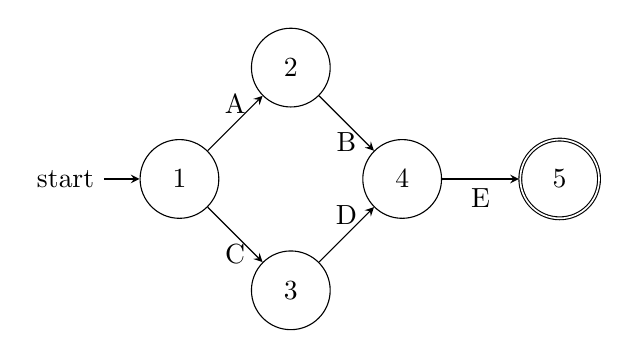
\begin{tikzpicture}[->, >=stealth, node distance=2cm, state/.style={circle, draw, minimum size=1cm}]

		\node[state, initial] (1) {1};
		\node[state] (2) [above right of=1] {2};
		\node[state] (3) [below right of=1] {3};
		\node[state] (4) [below right of=2] {4};
		\node[state, accepting] (5) [right of=4] {5};

		\path
		(1) edge node[above] {A} (2)
				edge node[below] {C} (3)
		(2) edge node[below] {B} (4)
		(3) edge node[above] {D} (4)
		(4) edge node[below] {E} (5);

		\end{tikzpicture}
		\caption{Diagrama de precedencia de actividades}
	\end{center}
\end{figure}


\begin{enumerate}
	\item[a)] Suponga el siguiente cuadro de duraciones para cada actividad.

		\begin{center}
			\begin{tabular}{|c|ccccc|}
				\hline
				$Actividad$ & $A$ & $B$ & $C$ & $D$ & $E$ \\
				\hline
				Duración (días) & 3 & 4 & 2 & 6 & 3 \\
				\hline
			\end{tabular}
		\end{center}

		Determine la duración del proyecto y su camino crítico.


	\begin{figure}[H]
		\begin{center}
			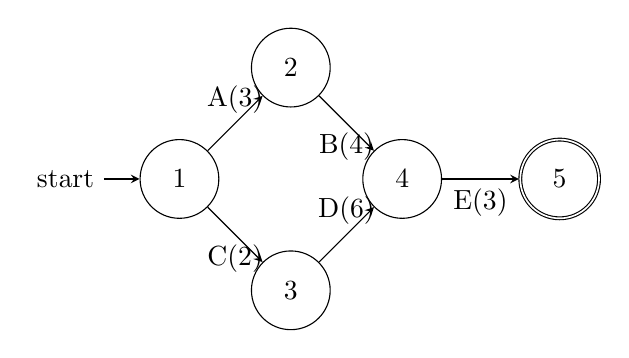
\begin{tikzpicture}[->, >=stealth, node distance=2cm, state/.style={circle, draw, minimum size=1cm}]

			\node[state, initial] (1) {1};
			\node[state] (2) [above right of=1] {2};
			\node[state] (3) [below right of=1] {3};
			\node[state] (4) [below right of=2] {4};
			\node[state, accepting] (5) [right of=4] {5};

			\path
			(1) edge node[above] {A(3)} (2)
					edge node[below] {C(2)} (3)
			(2) edge node[below] {B(4)} (4)
			(3) edge node[above] {D(6)} (4)
			(4) edge node[below] {E(3)} (5);

			\end{tikzpicture}
			\caption{Diagrama de precedencia de actividades con duración}
		\end{center}
	\end{figure}

	Se calcula la tabla de tiempos de inicio early ($E_i$) y late ($L_i$) de cada actividad.

	\begin{center}
		\begin{tabular}{|@{\hspace{0.3cm}}c@{\hspace{0.3cm}}|@{\hspace{0.3cm}}c@{\hspace{0.3cm}}|@{\hspace{0.3cm}}c@{\hspace{0.3cm}}|}
			\hline
			$t$ & $E_i$ & $L_i$ \\
			\hline
			1 & 0 & 0 \\
			2 & 3 & 4 \\
			3 & 2 & 2 \\
			4 & 8 & 8 \\
			5 & 11 & 11 \\
			\hline
		\end{tabular}
	\end{center}

	Una vez sabemos los tiempos de inicio early y late de cada actividad, calculamos los tiempos de holgura para encontrar el camino crítico.


	\begin{center}
		\begin{tabular}{|c|c|c|c|c|c|c|}
			\hline
			Tarea & $R_{ij}$ & $D_{ij}$ & $E_i$ & $L_j$ & $H_{ij}$ & Crítico\\
			A & $1\longrightarrow 2$ & 3 & 0 & 4 & 1 & \\
			B & $2\longrightarrow 4$ & 4 & 3 & 8 & 1 & \\
			C & $1\longrightarrow 3$ & 2 & 0 & 2 & 0 & X \\
			D & $3\longrightarrow 4$ & 6 & 2 & 8 & 0 & X \\
			E & $4\longrightarrow 5$ & 3 & 8 & 11 & 0 & X \\
			\hline
		\end{tabular}
	\end{center}

	Por lo tanto se establece que el camino crítico es C$\longrightarrow$ D$\longrightarrow$ E y la duración del proyecto es de 11 días.\\

	\item[b)] Suponga que no se conoce la duración de las actividades de forma determinista pero se estiman los siguientes tiempos optimista ($t_o$), más probable ($t_m$) y pesimista ($t_p$).

		\begin{center}
			\begin{tabular}{|c|c@{\hspace{0.3cm}}c@{\hspace{0.3cm}}c|}

					\hline
					$Actividad$ & $t_o$ & $t_m$ & $t_p$ \\
					\hline
					A & 2 & 5 & 8 \\
					B & 1 & 4 & 6 \\
					C & 2 & 2 & 3 \\
					D & 4 & 6 & 9 \\
					E & 3 & 5 & 7 \\
					\hline
			\end{tabular}
	\end{center}

	Determine la duración estimada del proyecto y su varianza, así como su camino crítico.\\

	Como en este caso no se conoce la duración de las actividades de forma determinista, se usará el método PERT para calcular la duración estimada del proyecto y su varianza. Una vez calculados los tiempos de duración de cada actividad, se calcula el camino crítico y la duración del proyecto por el método CPM. Para ello se calculan los tiempos de inicio early ($E_i$) y late ($L_i$) de cada actividad.

	Fórmula de la duración estimada:
	\begin{align*}
		D_e = \frac{t_o + 4t_m + t_p}{6} \\ \\
	\end{align*}

	Fórmula de la varianza:
	\begin{align*}
		\sigma^2 = \frac{(t_p - t_o)^2}{36}
	\end{align*}

	Con estos datos se calcula la duración estimada y la varianza de cada actividad creando la nueva tabla de duraciones que se usará con el método CPM.

	\begin{center}
		\begin{tabular}{|c|c@{\hspace{0.3cm}}c|}

				\hline
				$Actividad$ & $D_e$ & $\sigma^2$ \\
				\hline
				A & 5 & 1 \\
				B & 3.83 & 0.69 \\
				C & 2.17 & 0.03 \\
				D & 6.17 & 0.69 \\
				E & 5 & 0.44 \\
				\hline
		\end{tabular}
	\end{center}

	Con estos nuevos datos se calcula la holgura de cada actividad y se obtiene el camino crítico y la duración del proyecto.

	\begin{center}
		\begin{tabular}{|c|c|c|c|c|c|c|}
			\hline
			Tarea & $R_{ij}$ & $D_{ij}$ & $E_i$ & $L_j$ & $H_{ij}$ & Crítico\\
			A & $1\longrightarrow 2$ & 5 & 0 & 5 & 0 & X \\
			B & $2\longrightarrow 4$ & 3.83 & 5 & 8.83 & 0 & X \\
			C & $1\longrightarrow 3$ & 2.17 & 0 & 2.66 & 0.49 & \\
			D & $3\longrightarrow 4$ & 6.17 & 2.17 & 8.83 & 0.49 & \\
			E & $4\longrightarrow 5$ & 5 & 8.83 & 13.83 & 0 & X \\
			\hline
		\end{tabular}
	\end{center}

	Por lo tanto se establece que el camino crítico es A$\longrightarrow$ B$\longrightarrow$ E y se estima que la duración del proyecto sea de 13.83 días con una varianza de 2.13 días para el camino crítico.

\end{enumerate}

\section{La realización de un proyecto viene especificado por el siguiente orden de las actividades:}

	\begin{align*}
		A &\longrightarrow C \\
		B, C &\longrightarrow E \\
		D &\longrightarrow F \\
	\end{align*}
	La duración de las actividades no se conoce de forma determinista pero se estiman los siguientes tiempos optimista, medio y pesimista. Determine la duración estimada del proyecto y su varianza.

	\begin{center}
		\begin{tabular}{|c|c@{\hspace{0.3cm}}c@{\hspace{0.3cm}}c|}
			\hline
			$Actividad$ & $t_o$ & $t_m$ & $t_p$ \\
			\hline
			A & 3 & 5 & 10 \\
			B & 2 & 4 & 6 \\
			C & 2 & 2 & 2 \\
			D & 4 & 7 & 9 \\
			E & 4 & 5 & 7 \\
			F & 3 & 6 & 10 \\
			\hline
		\end{tabular}
	\end{center}
Primeramente vamos a generar el diagrama de precedencia de actividades.

	\begin{center}
		\begin{tikzpicture}[->, >=stealth, node distance=2cm, state/.style={circle, draw, minimum size=1cm}]

		\node[state, initial] (1) {1};
		\node[state] (2) [above right of=1] {2};
		\node[state] (3) [below right of=2] {3};
		\node[state] (4) [below of=3] {4};
		\node[state, accepting] (5) [right of=3] {5};

		\path
		(1) edge node[above] {A} (2)
				edge node[below] {B} (3)
				edge node[below] {D} (4)
		(2) edge node[above] {C} (3)
		(3) edge node[above] {E} (5)
		(4) edge node[above] {F} (5)

		\end{tikzpicture}
	\end{center}


De igual forma que en el ejercicio anterior, se calcula la duración estimada y la varianza de cada actividad creando la nueva tabla de duraciones que se usará con el método CPM.

	\begin{center}
		\begin{tabular}{|c|c@{\hspace{0.3cm}}c|}

				\hline
				$Actividad$ & $D_e$ & $\sigma^2$ \\
				\hline
				A & 5.5 & 1.36 \\
				B & 4 & 0.44 \\
				C & 2 & 0 \\
				D & 6.83 & 0.69 \\
				E & 5.17 & 0.25 \\
				F & 6.17 & 1.36 \\
				\hline
		\end{tabular}
	\end{center}

	Calculamos los tiempos de inicio early ($E_i$) y late ($L_i$) de cada actividad.
	\begin{center}
		\begin{tabular}
			{|@{\hspace{0.3cm}}c@{\hspace{0.3cm}}|@{\hspace{0.3cm}}c@{\hspace{0.3cm}}|@{\hspace{0.3cm}}c@{\hspace{0.3cm}}|}
			\hline
			$t$ & $E_i$ & $L_i$ \\
			\hline
			1 & 0 & 0 \\
			2 & 5.5 & 5.83 \\
			3 & 7.5 & 7.83 \\
			4 & 6.83 & 6.83 \\
			5 & 13 & 13 \\
			\hline
		\end{tabular}
	\end{center}

	Con estos nuevos datos se calcula la holgura de cada actividad y se obtiene el camino crítico y la duración del proyecto.

	\begin{center}
		\begin{tabular}{|c|c|c|c|c|c|c|}
			\hline
			Tarea & $R_{ij}$ & $D_{ij}$ & $E_i$ & $L_j$ & $H_{ij}$ & Crítico\\
			A & $1\longrightarrow 2$ & 5.5 & 0 & 5.83 & 0.33 & \\
			B & $1\longrightarrow 3$ & 4 & 0 & 7.83 & 3.83 & \\
			C & $2\longrightarrow 3$ & 2 & 5.5 & 7.83 & 0.33 & \\
			D & $1\longrightarrow 4$ & 6.83 & 0 & 6.83 & 0 & X \\
			E & $3\longrightarrow 5$ & 5.17 & 7.5 & 13 & 0.33 & \\
			F & $4\longrightarrow 5$ & 6.17 & 6.83 & 13 & 0 & X \\
			\hline
		\end{tabular}
	\end{center}

	El camino crítico en este caso es D$\longrightarrow$ F y la duración estimada del proyecto es de 13 días con una varianza de 2.05 días.

\newpage
Yo, Miguel Ángel Dorado Maldonado, a día 22 de diciembre de 2024, declaro bajo mi palabra de honor que el trabajo aquí entregado es de mi autoría y originalidad. Asimismo, confirmo que no he utilizado recursos externos que no hayan sido debidamente citados ni recibido ayuda no autorizada en su realización.
\end{document}
